\documentclass[
  aps,
  prl,
  reprint,
  superscriptaddress,
  nofootinbib,
  longbibliography,
  floatfix
]{revtex4-2}

\usepackage{amsmath,amssymb,bm}
\usepackage{graphicx}
\usepackage{xcolor}
\usepackage{microtype}
\usepackage{hyperref}
\hypersetup{
  colorlinks=true,
  allcolors=blue!55!black,
  pdftitle={Basis-Dependent Sparsity and Energy Recovery in a Strongly Correlated [2Fe--2S] Active Space},
  pdfauthor={Anonymous Authors},
  pdfsubject={Variational active-space electronic structure and determinant compressibility},
  pdfkeywords={iron-sulfur cluster, variational energy, configuration interaction, natural orbitals, wave-function compression}
}

\newcommand{\Eh}{E_{\mathrm h}}
\newcommand{\cas}{\mathrm{CAS}(30e,20o)}
% Frozen numerical values generated by analysis/build_results_tex.py.
\newcommand{\FinalEnergy}{-116.60560912042631}
\newcommand{\FinalResidual}{6.9016\times10^{-7}}
\newcommand{\BenchmarkKFiveTwelveCoupling}{1.2105313}
\newcommand{\BenchmarkKFiveTwelveTail}{-0.6052656}
\newcommand{\NaturalKFiveTwelveRelaxedEnergy}{-116.486260278799}
\newcommand{\NaturalKFiveTwelveRelaxedErrorMilli}{119.349}
\newcommand{\NaturalKFiveTwelveRelaxationGainMilli}{49.634}
\newcommand{\NaturalKFiveTwelveProjectedResidual}{1.68\times10^{-13}}
\newcommand{\NaturalKFiveTwelveFullResidual}{0.311254}
\newcommand{\NaturalKFiveTwelveIndependentDifference}{5.68\times10^{-14}}
\newcommand{\NaturalReplayTrace}{29.999999987374895}
\newcommand{\NaturalReplayExpectedTrace}{30.000000000000426}
\newcommand{\NaturalReplayTraceError}{1.26\times10^{-8}}
\newcommand{\NaturalReplayRDMSymmetry}{0}
\newcommand{\NaturalReplayRDMOffDiagonal}{2.27\times10^{-11}}
\newcommand{\NaturalReplayRDMReferenceDifference}{6.27\times10^{-10}}
\newcommand{\NaturalReplayOccupationsDifference}{6.27\times10^{-10}}
\newcommand{\LateBasisSentence}{At \(K=4{,}194{,}304\), the natural-orbital projection increases \(W_K\) from 0.985678 to 0.999776 and reduces \(\Delta E_K\) from 17.705 to \(0.3488\,\mathrm{m}\Eh\); its residual nevertheless remains \(2.72\times10^{-2}\,\Eh\).}


\begin{document}

\title{Basis-Dependent Sparsity and Energy Recovery in a Strongly Correlated [2Fe--2S] Active Space}

\author{Anonymous Authors}
\affiliation{Affiliations withheld during scientific review}

\begin{abstract}
Orbital rotations redistribute determinant amplitudes without changing a state, so
coefficient weight need not certify energy.  For the \(\cas\) [2Fe--2S]
Hamiltonian, a Davidson Ritz vector gives \(E=\FinalEnergy\,\Eh\),
\(184\,\mu\Eh\) below reported HCI, with residual
\(\FinalResidual\,\Eh\).  Natural orbitals raise the top-512 norm from 0.191
to 0.769, but leave \(169\,\mathrm{m}\Eh\) error.  Fixed-support and
Hamiltonian-guided controls separate basis, coefficient, and support effects.
Energy compressibility requires Hamiltonian contraction, not fidelity alone.
\end{abstract}

\maketitle

The compression of a correlated electronic state is inseparable from the
choice of representation.  Selected configuration-interaction (SCI) methods
construct compact determinant spaces using estimates of Hamiltonian-mediated
importance~\cite{holmes2016,sharma2017,zhang2025}, whereas state-sampling
workflows may first rank observed configurations by squared coefficient and
then diagonalize the Hamiltonian in the retained subspace~\cite{yoo2026}.
These operations answer different questions.  The \(K\) largest coefficients
give the best \(K\)-term approximation in Hilbert-space norm for a fixed
orbital basis, but neither that support nor its inherited coefficients are
guaranteed to minimize the energy.  Moreover, an active--active orbital
rotation leaves the physical state unchanged while generally redistributing
its determinant amplitudes.

This distinction is especially important for iron--sulfur clusters, whose
coupled high-spin centers generate dense multireference manifolds and severe
entanglement~\cite{sharma2014,li2017}.  The
\([\mathrm{Fe}_2\mathrm{S}_2(\mathrm{SCH}_3)_4]^{2-}\) model in a
\(\cas\) active space is consequently used to assess DMRG, neural
wave functions, SCI, and quantum-classical methods~\cite{li2017,ma2025,yoo2026}.
Here we first obtain a lower explicit variational energy for this Hamiltonian.
We then use the saved state to ask a representation-resolved question: how do
orbital adaptation, coefficient relaxation, and Hamiltonian-guided support
selection change the energy attainable with a finite determinant expansion?

\textit{Hamiltonian and Ritz calculation.---}
We consider 30 electrons in 20 orthonormal spatial orbitals, restricted to
\(M_S=0\), with
\begin{equation}
 \hat H=\sum_{pq\sigma}h_{pq}a^{\dagger}_{p\sigma}a_{q\sigma}
 +\frac{1}{2}\sum_{pqrs\sigma\tau}g_{pqrs}
 a^{\dagger}_{p\sigma}a^{\dagger}_{r\tau}a_{s\tau}a_{q\sigma}.
 \label{eq:hamiltonian}
\end{equation}
The spin-string coefficient tensor has shape
\(\binom{20}{15}\!\times\!\binom{20}{15}=15{,}504^2\), or
\(240{,}374{,}016\) real amplitudes.  We use the archived benchmark
FCIDUMP~\cite{qatHamiltonian}.  A second FCIDUMP distributed with the QMB
models~\cite{qmbModels,li2017} is related to it by an orthogonal orbital
rotation: the transformed one-electron tensor agrees to
\(3.55\times10^{-14}\,\Eh\) elementwise, and the complete two-electron tensor
has root-mean-square and maximum discrepancies
\(3.08\times10^{-15}\,\Eh\) and \(1.21\times10^{-13}\,\Eh\), respectively.

We minimize the Rayleigh quotient in the complete configuration-interaction
space \emph{within} this active space and spin sector,
\begin{equation}
 E[\bm c]=\frac{\bm c^{\mathsf T}H\bm c}{\bm c^{\mathsf T}\bm c},\qquad
 \rho(\bm c)=\frac{\lVert H\bm c-E[\bm c]\bm c\rVert_2}
 {\lVert\bm c\rVert_2},
 \label{eq:ritz}
\end{equation}
using a diagonally preconditioned, restarted Davidson iteration~\cite{davidson1975}
and matrix-free Slater--Condon contractions in PySCF~\cite{sun2018,sun2020}.
Atomic checkpoints permit wider-subspace restarts without replacing the
explicit state by extrapolated energies.  The final production stage used a
64-vector maximum subspace, 160 updates, an energy threshold
\(10^{-13}\,\Eh\), and residual target \(10^{-8}\,\Eh\).  The full staged
simulation, initialization, environment, and executable commands are given in
the Supplemental Material~\cite{supplement}.

\begin{figure*}[t]
  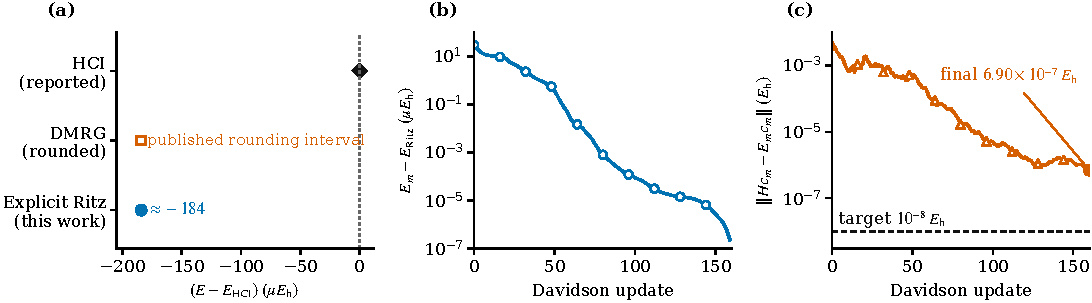
\includegraphics[width=\textwidth]{figures/figure1.pdf}
  \caption{\textbf{Explicit variational energy and numerical convergence.}
  (a) Energies relative to the reported HCI entry.  The DMRG segment denotes
  only the interval that rounds to the published digits.  (b) Positive
  Ritz-energy difference from the final saved state during the production
  stage.  (c) Residual norm of the same iterates.  The final point remains
  above the preset \(10^{-8}\,\Eh\) target.}
  \label{fig:bound}
\end{figure*}

The saved vector has squared norm \(0.999999999999999\) and direct Rayleigh
energy and residual
\begin{equation}
 \begin{aligned}
 E_{\star}&=\FinalEnergy\,\Eh,\\
 \rho_{\star}&=\FinalResidual\,\Eh .
 \end{aligned}
 \label{eq:result}
\end{equation}
This energy is approximately \(184\,\mu\Eh\) below the reported HCI value
\(-116.605425\,\Eh\)~\cite{qatHCI}; the precision shown for that entry does
not support finer comparison.  It lies in the rounding interval of the
published DMRG value \(-116.6056091\,\Eh\)~\cite{li2017,qmbModels}, so we
claim agreement with, not improvement over, DMRG
[Fig.~\ref{fig:bound}(a)].  A fresh-process
Hamiltonian application reproduces Eq.~(\ref{eq:result}); a separate
one- and two-particle density-matrix contraction agrees within
\(5.97\times10^{-13}\,\Eh\), and
\(\langle\hat S^2\rangle=2.86\times10^{-9}\).  The Davidson convergence flag
is false because \(\rho_\star\) exceeds the preset target
[Fig.~\ref{fig:bound}(c)].  Nevertheless, the explicit Rayleigh quotient is a
variational upper bound to the lowest eigenvalue in the stated sector.  We do
not infer a two-sided error bar from the residual.

\textit{Representation-resolved compression.---}
We compare the benchmark orbital basis, denoted \(b=\mathrm{B}\), with an
a posteriori natural-orbital basis \(b=\mathrm{N}\).  Diagonalizing the
spin-summed one-particle density matrix gives
\(\gamma U=U\,\mathrm{diag}(n_p)\).  We transform both the integrals and the
complete CI tensor by the same \(U\); direct contractions before and after the
rotation preserve the norm, energy, and residual to
\(1.4\times10^{-14}\), \(3.13\times10^{-13}\,\Eh\), and
\(1.12\times10^{-16}\,\Eh\), respectively.  Thus the two coefficient tensors
are representations of the same physical Ritz state, not separate electronic
solutions.

For each representation, \(P_K^{(b)}\) retains the \(K\) largest values of
\(|c_I^{(b)}|\).  We define
\begin{equation}
 \begin{aligned}
 W_K^{(b)}&=\langle c|P_K^{(b)}|c\rangle,\\
 |\phi_K^{(b)}\rangle&=\frac{P_K^{(b)}|c\rangle}{\sqrt{W_K^{(b)}}},\\
 \Delta E_K^{(b)}&=\langle\phi_K^{(b)}|H|\phi_K^{(b)}\rangle-E_\star .
 \end{aligned}
 \label{eq:topk}
\end{equation}
Every projected energy and residual in Fig.~\ref{fig:compression} is obtained
from a new full Hamiltonian contraction.  No energy is estimated from discarded
weight.  The natural orbitals strongly concentrate the norm: at \(K=64\),
\(W_K\) rises from 0.0755 to 0.4181; at \(K=512\), it rises from 0.1913 to
0.7685.  The energetic improvement is real but not commensurate with the
fidelity: the natural-orbital \(K=512\) projection remains
\(168.98\,\mathrm{m}\Eh\) above \(E_\star\), with residual
\(0.473\,\Eh\).  \LateBasisSentence

\begin{figure*}[t]
  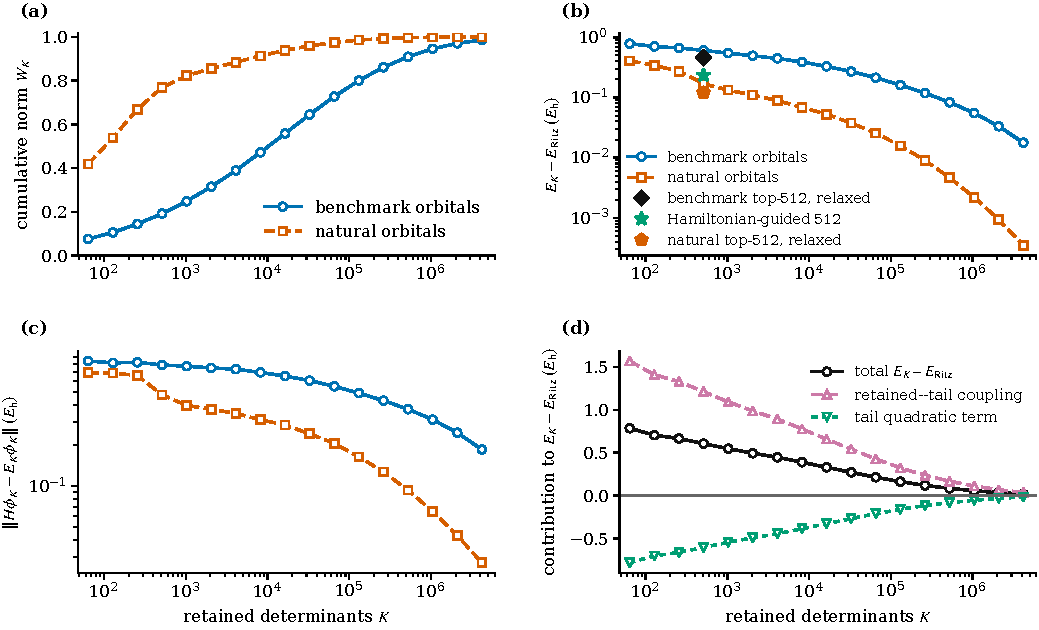
\includegraphics[width=\textwidth]{figures/figure2.pdf}
  \caption{\textbf{Orbital adaptation, coefficient relaxation, and support
  choice.}  (a) Cumulative norm of amplitude-ranked projections in the
  benchmark and natural-orbital representations.  (b) Directly contracted
  energy errors.  The diamond and pentagon are exact ground states on the
  benchmark- and natural-basis top-512 supports, respectively; the star is an
  independently constructed Hamiltonian-guided 512-determinant support in the
  benchmark basis.
  (c) Full-space residuals of the fixed-coefficient projections.
  (d) Gauge-invariant decomposition of the benchmark-basis error into removed
  retained--tail coupling and tail quadratic terms.  The latter is negative;
  their sum is the positive projected-state error.}
  \label{fig:compression}
\end{figure*}

To isolate what amplitude pruning leaves unresolved, we perform two
\(K=512\) controls in the benchmark basis.  The inherited top-512 coefficients
give \(-116.0003434451\,\Eh\).  Exact diagonalization on that \emph{same}
support lowers the energy by \(145.97\,\mathrm{m}\Eh\), to
\(-116.1463085705\,\Eh\).  An independently constructed, Hamiltonian-guided
512-determinant support, followed by exact subspace diagonalization, gives
\(-116.3704626758\,\Eh\).  Its advantage over the inherited top-512 state is
\(370.12\,\mathrm{m}\Eh\), but it remains \(235.15\,\mathrm{m}\Eh\) above
\(E_\star\).  A fermionic-operator reference implementation and a PySCF
full-space embedding agree on both rediagonalized energies within
\(3.2\times10^{-13}\,\Eh\).  Their projected-support residuals are below
\(2.5\times10^{-13}\,\Eh\), whereas their full-space residuals are 0.558 and
0.215\,\(\Eh\).  These controls establish coefficient stationarity only on
their stated supports; they neither identify a globally optimal support nor
bound a fully adaptive SCI calculation.

The a posteriori natural-orbital top-512 projection is lower still,
\(-116.4366261444\,\Eh\), by \(66.16\,\mathrm{m}\Eh\) relative to the
Hamiltonian-guided benchmark-basis control.  Rediagonalizing its unchanged
support gains another \(\NaturalKFiveTwelveRelaxationGainMilli\,\mathrm{m}\Eh\),
giving \(\NaturalKFiveTwelveRelaxedEnergy\,\Eh\).  The projected residual is
\(\NaturalKFiveTwelveProjectedResidual\,\Eh\), but the full-space residual is
still \(\NaturalKFiveTwelveFullResidual\,\Eh\): coefficient stationarity does
not remove coupling to excluded determinants.  These comparisons show how
strongly the one-particle representation can affect a fixed determinant
budget.  They are not a constructive sparse-solver benchmark, because the
natural orbitals were obtained from the complete Ritz state.

The missing energetic contribution can be resolved without reference to the
arbitrary zero of energy.  Let \(A=H-E_\star I\),
\(p=P_Kc\), \(q=(I-P_K)c\), and \(W=\langle p|p\rangle\).  Since
\(\langle c|A|c\rangle=0\),
\begin{equation}
 \Delta E_K=
 \underbrace{-\frac{2\,\mathrm{Re}\langle p|A|q\rangle}{W}}_{C_K}
 +
 \underbrace{-\frac{\langle q|A|q\rangle}{W}}_{T_K}.
 \label{eq:decomposition}
\end{equation}
Using the directly contracted \(E_\star\), \(E_K\), and
\(\langle c|H|\phi_K\rangle\), we algebraically reconstruct both terms; their
maximum floating-point recombination error is
\(6.1\times10^{-14}\,\Eh\).  In the benchmark representation at \(K=512\),
the removed retained--tail coupling contributes
\(C_K=\BenchmarkKFiveTwelveCoupling\,\Eh\), while the tail quadratic term
contributes \(T_K=\BenchmarkKFiveTwelveTail\,\Eh\); their cancellation leaves
the \(0.60527\,\Eh\) error of the normalized projection.  The same pattern
persists across the evaluated supports [Fig.~\ref{fig:compression}(d)].  Large
discarded contributions can therefore cancel in the full state even when the
discarded norm is small; \(W_K\) alone contains neither matrix elements nor
their signs.

Our conclusion is deliberately narrower than a claim about all SCI methods.
Natural orbitals substantially improve determinant sparsity for this state,
and Hamiltonian-based coefficient and support optimization substantially lower
sparse-state energies.  Yet in both tested representations the mapping from
retained norm to energy error must be established by Hamiltonian contraction.
For sampling-based subspace methods, this diagnoses the amplitude-ranking step,
not the subsequent subspace diagonalization.  More broadly, fidelity, support
choice, coefficient stationarity, and full-space stationarity are distinct
properties and should be reported separately.

In summary, a reproducible Davidson calculation yields an explicit \(\cas\)
variational energy below the reported HCI entry and consistent with rounded
DMRG.  Exact orbital transformation and sparse controls then show that orbital
adaptation changes how compact the coefficient vector appears without turning
amplitude weight into an energetic certificate.  The result supplies both a
lower classical reference and a representation-aware protocol for testing
sparse classical and quantum ansatzes.

\bibliography{references}

\end{document}
